% 手拉手模型（基础版）：两个共顶点等腰三角形 △OAB、△OCD（顶角均约 50°）
% 红色虚线 AC、BD 即"手拉手"两段，应等长
\documentclass[tikz,border=4pt]{standalone}
\usetikzlibrary{calc, decorations.markings}
\begin{document}
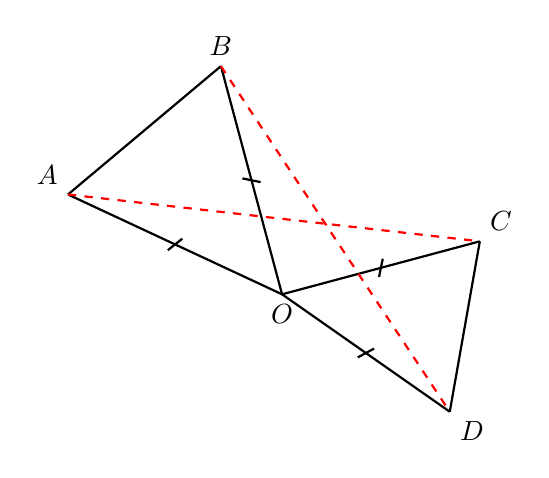
\begin{tikzpicture}[scale=1.0, thick,
  tick/.style={postaction={decorate, decoration={markings,
    mark=at position 0.5 with {\draw (-1.5pt,-3pt) -- (1.5pt,3pt);}}}}]

  \coordinate (O) at (0, 0);
  % △OAB: 顶角 ∠AOB=50°，OA=OB=3，整体偏左上
  % 以 OA 方向 155°、OB 方向 105° 配置
  \coordinate (A) at ({3*cos(155)}, {3*sin(155)});
  \coordinate (B) at ({3*cos(105)}, {3*sin(105)});
  % △OCD: 顶角 ∠COD=50°，OC=OD=2.6，偏右下
  \coordinate (C) at ({2.6*cos(15)}, {2.6*sin(15)});
  \coordinate (D) at ({2.6*cos(-35)}, {2.6*sin(-35)});

  % 两腰用同种 tick 标"等长"
  \draw[tick] (O) -- (A);
  \draw[tick] (O) -- (B);
  \draw (A) -- (B);
  \draw[tick] (O) -- (C);
  \draw[tick] (O) -- (D);
  \draw (C) -- (D);

  % 手拉手两段
  \draw[red, dashed] (A) -- (C);
  \draw[red, dashed] (B) -- (D);

  \node[below]       at (O) {$O$};
  \node[above left]  at (A) {$A$};
  \node[above]       at (B) {$B$};
  \node[above right] at (C) {$C$};
  \node[below right] at (D) {$D$};
\end{tikzpicture}
\end{document}
